\documentclass[a0,portrait,brazil]{a0poster}
\usepackage[utf8]{inputenc}

\usepackage{multicol} 
\columnsep=100pt
\columnseprule=3pt

\usepackage[svgnames]{xcolor} 
\usepackage{times}
\usepackage{scalefnt}
\usepackage{comment}
\usepackage{amsmath,environ}
\usepackage{float}
\usepackage{amsfonts} 
\DeclareMathAlphabet\bfmathcal{OMS}{cmsy}{b}{n}

\usepackage{graphicx}
\graphicspath{{figures/}}
\usepackage{booktabs} 
\usepackage[font=small,labelfont=bf]{caption}
\usepackage{amsfonts, amsmath, amsthm, amssymb}
\usepackage{wrapfig} 
\definecolor{ku}{RGB}{144,26,30}
\definecolor{ku-yellow}{RGB}{255,249,25}
\usepackage{pgf,tikz}
\usetikzlibrary{arrows,automata,positioning}
\usetikzlibrary{arrows,shapes.gates.logic.US,shapes.gates.logic.IEC,calc}
\renewcommand\tablename{Tabela}
\renewcommand\figurename{Figura}
\usepackage{lipsum}

 \usepackage{eso-pic}
               \newcommand\BackgroundIm{
               \put(56,15){
               \parbox[b][\paperheight]{\paperwidth}{%
               \vfill
               \centering
               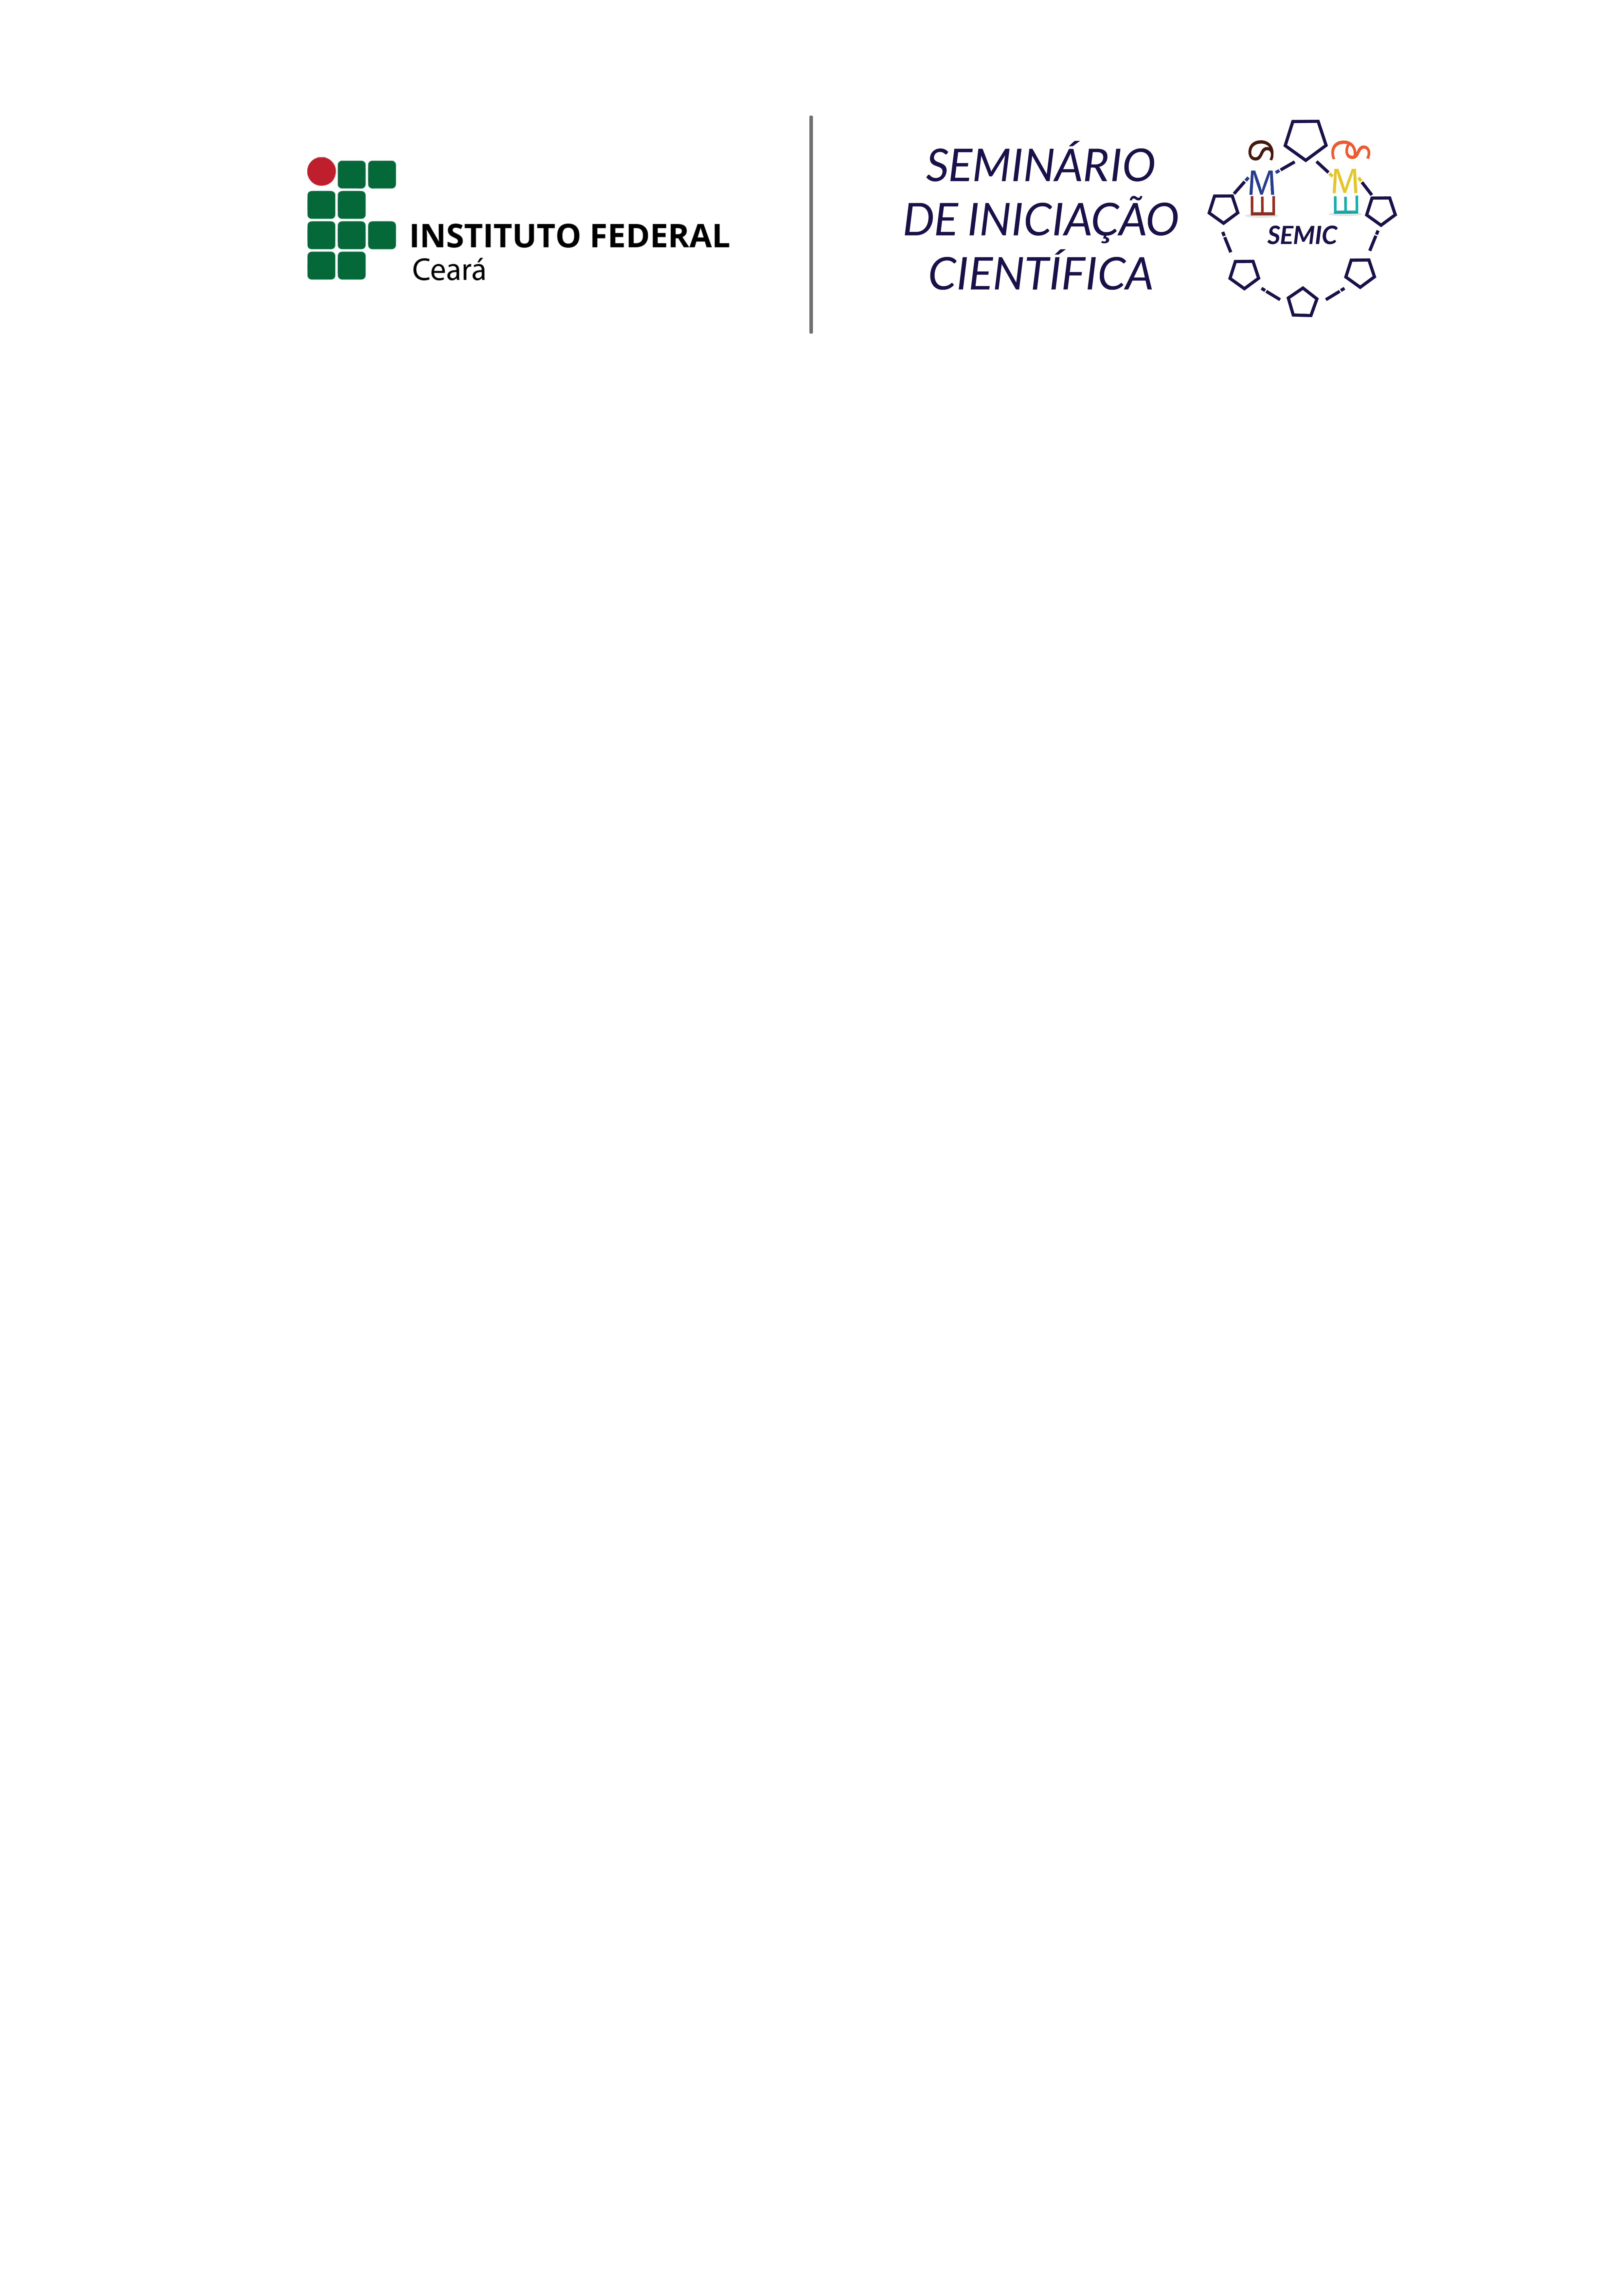
\includegraphics[height=\paperheight,width=\paperwidth,
               keepaspectratio]{back2.png}
               \vfill
               }}}
\DeclareMathOperator*{\argmin}{arg\,min}


\hyphenation{satisfa-tibilidade}
\hyphenation{exa-tamente}
\hyphenation{esco-lhendo}


\begin{document}
 \AddToShipoutPicture*{\BackgroundIm}

\begin{minipage}[t]{0.97\linewidth}
\vspace{10cm}
\begin{center}
\vspace{1cm} 
\Huge \color{black} \textbf{ENSINO  DE  ROBÓTICA  NAS  ESCOLAS  PÚBLICAS  UTILIZANDO  MATERIAIS  RECICLADOS  E  PRINCÍPIOS  DE  APRENDIZAGEM  BASEADA  EM  PROJETOS} \color{Black}\\ [0.5cm] 
%% \Huge \color{black} \textbf{} \color{Black}\\ [1cm]
\Large \textbf{Vitor Veras de Moura}$^ {1}$, \textbf{Vinícius Ferreira da Silva}$^ {2}$, \textbf{Sandro César Silveira Jucá}$^ {3}$\\[0.2cm]
\large \text{$^{1}$Bolsista, Instituto Federal do Ceará - \textit {Campus Maracanaú}, vitorverasm@gmail.com}\\[0.2cm]
\large \text{$^{2}$Orientador, Instituto Federal do Ceará - \textit {Campus Maracanaú}, sandrojuca@ifce.edu.br}\\[0.2cm]
\end{center}

\end{minipage}
\vspace{1cm} 

\begin{multicols}{3} 

%--------------------------------------------
%	ABSTRACT
%--------------------------------------------
\color{black} 
\begin{large}
\section*{RESUMO}
O projeto proposto tem por objetivo a implementação de um projeto de robótica educacional em escolas públicas. O robô desenvolvido, utiliza-se dos conceitos da metarreciclagem, conceitos de IoT(Internet of Things) e da metodologia de Aprendizagem baseada em Projeto (ABP), o que visa incentivar a sustentabilidade e o reuso de componentes eletrônicos de forma a minimizar a geração de lixo. O projeto desenvolvido também promove a interdisciplinaridade entre as áreas comuns ensinadas nas escolas, tornando mais dinâmico e interativo o processo de aprendizagem.
\vspace{0.1cm}

\textbf{Palavras-Chave:} Robótica. Metarreciclagem. Educação.

%--------------------------------------------
%	INTRODUCTION
%--------------------------------------------
\color{black}
\section*{INTRODUÇÃO}
A robótica educacional caracteriza-se por promover a interdisciplinaridade, reunindo várias áreas de ensino, como informática, eletrônica, física, matemática entre outras, considerando os diversos componentes envolvidos no processo de ensino-aprendizagem, como motores, atuadores e sensores. Geralmente, estes componentes são controlados por hardware e softwares livres que permitem manipular o funcionamento dos modelos montados, podendo assim, estimular o raciocínio lógico e a construção de novos conceitos relacionados à inclusão digital.
\medskip

A utilização de atividades de robótica educacional, demonstra a possibilidade de se abordar concretamente e de forma contextualizada os diversos conceitos utilizados nas práticas da sala de aula, possibilitando um maior interesse dos alunos fazendo com que estes despertem o seu lado pesquisador, afirmam \cite{robo3}, estabelecendo conexões entre os conteúdos, promovendo, desta maneira, a interdisciplinaridade, e estimulando o trabalho cooperativo \cite{robo1}.
\medskip

A aprendizagem baseada em projeto (ABP) visa trabalhar com os estudantes a resolução de problemas do mundo real, pode ser definida pela utilização de projetos baseados em uma questão, problema ou tarefa, que sejam motivadores e envolventes afim de ensinar conteúdos acadêmicos aos alunos \cite{abp}. Por outro lado, a IoT pode ser definida como um ecossistema onde tudo que apresenta conexão com a Internet e é aplicado em um processo ou produto pode ser interpretado como Internet das Coisas.
\medskip

A metarreciclagem surge então na necessidade da utilização do lixo eletrônico através de sua desconstrução ou reutilização, para assim, construir novos produtos. Os princípios da metarreciclagem têm por base a desconstrução de equipamentos em desuso, o uso de softwares livres, o uso de licenças abertas e a ação em rede, onde qualquer pessoa pode colaborar buscando meios para a reutilização do lixo eletrônico proporcionando a formação de ideias sobre a reapropriação de tecnologia objetivando a transformação social \cite{robo2}.
\medskip

O projeto visa então atrair o interesse de alunos de escolas públicas com o conceito da robótica educacional de baixo custo, junto ao de metarreciclagem. Experimentos práticos aliados à teoria das disciplinas convencionais como física e matemática, por exemplo, podem contribuir com o aprendizado dos alunos, principalmente aqueles que tem mais dificuldade.

%--------------------------------------------
%	METHODS
%--------------------------------------------
\color{black} 
\section*{METODOLOGIA}

O robô móvel proposto neste trabalho tem como objetivo seguir uma determinada linha de percurso circular. Isto foi possível através da reutilização de componentes eletrônicos retirados principalmente de impressoras e computadores em desuso. A Figura~\ref{fig:fig1} mostra a representação do esquema para a construção do robô móvel.
\medskip

\begin{figure}[H]
\centering
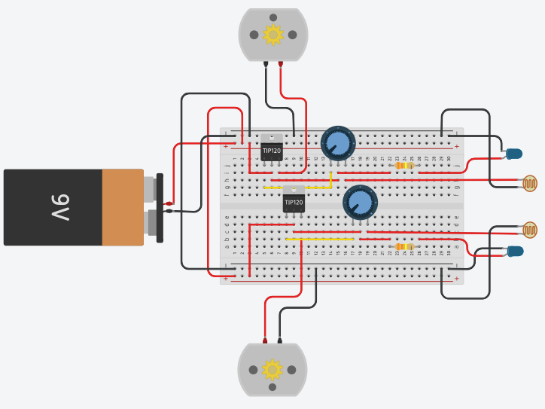
\includegraphics[width=.2\textwidth]{figures/SEMIC1.png}
\caption{Esquema dos componentes utilizados no projeto proposto}
\label{fig:fig1}
\end{figure}

Para a construção deste projeto foram utilizados dois TIPs-122, o TIP-122 é um transistor de potência e alto ganho, que recebe um sinal muito fraco na entrada chamado também como base e transforma-o em um sinal potente na saída seja ele o coletor ou emissor \cite{fairchild}. Dois potenciômetros de 100k utilizados para ajustar a resistência a ser passada para os LEDs, no intuito de aumentar ou diminuir a intensidade da luminosidade de ambos. Dois resistores de 360ohms utilizados principalmente para reduzir a corrente dos LEDs, e uma placa de circuito impresso utilizada para agregar os componentes eletrônicos do projeto.


%--------------------------------------------
%	CONCLUSIONS
%--------------------------------------------

\color{black}
\section*{RESULTADOS}

Como visto neste trabalho, o entendimento e uso da robótica educacional e da metarreciclagem em conjunto com a ABP no âmbito educacional, pode proporcionar aos alunos um contato mais aprofundado com a prática, aliado aos conceitos teóricos. Esses conceitos, como também a aplicação prática dos mesmos, promoveu a interdisciplinaridade em sala de aula. Esse projeto foi apresentado no Instituto Idear para estudantes de escolas públicas, os quais despertaram interesse para aprofundamento do tema e desenvolvimento de outros projetos relacionados.
\medskip

Na Figura~\ref{fig:fig2} é possível notar os componentes fundamentais para o funcionamento do robô móvel, sendo eles, dois LDRs (E) constituídos de um semicondutor de alta resistência dependente de luz, que ao receber uma grande quantidade de fótons vindos da luz incidente dos LEDs (F), eles absorvem os elétrons que melhoram sua condutibilidade, reduzindo assim sua resistência, ou seja, quando estes estiverem em contato com uma intensidade de luz grande, o motor do robô móvel será ativado e quando estiver com pouca intensidade de luz o motor irá parar. O robô consiste ainda em dois motores de 3V (G), uma bateria recarregável de 9V (H), um interruptor para ligar e desligar o robô (I) e por último uma placa recortada utilizada como base do projeto.
\medskip

\begin{figure}[H]
\centering
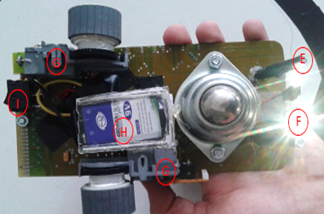
\includegraphics[width=.25\textwidth]{figures/SEMIC2.png}
\caption{Visão da parte traseira do projeto proposto}
\label{fig:fig2}
\end{figure}

\color{black}
\section*{CONSIDERAÇÕES FINAIS}

Como visto neste trabalho, o entendimento e uso da robótica educacional e da metarreciclagem em conjunto com a ABP e conceitos de IoT no âmbito educacional, pode proporcionar aos alunos um contato mais aprofundado com a prática, aliado aos conceitos teóricos. Esses conceitos, como também a aplicação prática dos mesmos, promoveu a interdisciplinaridade em sala de aula. Esse projeto foi apresentado no Instituto Idear para estudantes de escolas públicas, os quais despertaram interesse no aprofundamento do tema e em desenvolver outros projetos relacionados. 


%--------------------------------------------
%	REFERENCES
%--------------------------------------------
\vspace{-1cm}
\color{black}
\renewcommand{\refname}{REFERÊNCIAS}
%\nocite{*} % Print all references regardless of whether they were cited in the poster or not
\bibliographystyle{plain} % Plain referencing style
\bibliography{references} % Use the example bibliography file sample.bib

%--------------------------------------------
%	ACKNOWLEDGEMENTS
%--------------------------------------------

%----------------------------------------------------------------------------------------
\end{large}
\end{multicols}
\end{document}
